\chapter{绪论}\label{cha:introduction}


% 江恩慧 2022本子
长期的研究与探索,流域系统概念逐渐明晰。程国栋和李新(2015)在“黑河流域生态-水文过程集成研究”中提出了流域科学的概念,将流域视为地球系统的缩微,考虑水文和生态系统的自组织性如何影响流域系统的功能,以及人的因素如何被集成到流域水文学和流域生态学中。傅伯杰(2017)指出亟需聚焦人地系统耦合机理与调控途径,揭示黄河流域人水关系演变及社会-水文-生态系统动态。

\section{研究背景与意义}\label{sec:background}
\subsection{人与自然相互作用:人地关系的研究前沿}

% 帮王老师写的综述:人地系统结构与可持续V2
在人类活动的强烈影响下,地球进入了“人类世”的新纪元。
这意味着人类对地球改造的程度和后果可以与传统意义上的地质营力产生的影响相匹敌,成为环境变化的重要驱动力\cite{lenton2019, lewis2015, lewis2018}。
过去数世纪以来,这种来自人类的改造和控制已经让气候变化、生物多样性损失和氮循环等关键地球系统生态过程超越了危险的“地球界限”,导致了众多资源、生态和环境问题\cite{steffen2015}。
如何在满足人类发展需求的同时,持续地保障地球生命支持系统的基本结构和功能,实现可持续发展,已成为学术界和社会各界广泛关注的重大科学和决策问题\cite{wu2014}。
人与自然地理环境密不可分,理解现代环境变化机理、持续地保障地球生命支持系统的基本结构和功能需要发展人地系统整体的方法,耦合自然与人文过程,探讨变化环境下的系统耦合机制\cite{fu2015}。

在涉及人地关系综合研究的学科中,地理学以地域为单元,着重研究地球表层人与自然的相互影响和反馈作用,对人地关系的认识一直是地理学的研究核心\cite{wu1991}。
钱学森先生倡导的“地球表层学”、吴传钧先生提出的“人地关系地域系统”、黄秉维先生倡导“陆地表层系统科学”等学说都强调了人与自然相互作用形成的人地关系复合系统,也就是人与地在特定的地域中相互联系、相互作用而形成的一种动态结构。
面对环境问题的复杂性,不同空间尺度上人类活动与自然环境的耦合关系正在成为国际学界的主流话题。例如,美国科学基金会(NSF)于2001年开展了自然与人类耦合系统动力学(Dynamics of Coupled Natural and Human Systems-CNH)研究计划。该计划于2019年发展为CNH2-社会-环境综合系统动力学计划(Dynamics of Integrated Socio-Environmental Systems)。此外,“未来地球”科学计划旨在推动自然科学与社会科学研究成果共同为可持续发展服务\cite{fu2015}。
% https://www.nsf.gov/news/special_reports/announcements/110619.jsp
在人类活动影响力不断增强的背景下,制定区域可持续发展战略必须深入了解人类赖以生存的地球环境系统与人类系统之间相互作用的基本过程。因此,关注人地系统演变及其机制的人地系统动力学成为研究的重要方向\cite{fu2022}。

\subsection{人-水系统耦合:流域治理的科学基础}

% 开题报告
水是连接自然系统和社会系统的纽带,水循环过程是生态过程和社会发展的重要驱动力,人-水系统是以水循环为纽带将人文系统与水系统联系在一起的复合系统,是在流域尺度紧密相连的开放巨系统,也是典型的人与自然耦合系统\cite{li2007}。
% 于璐 本子
早在2013年,国际水文科学协会就启动十年科学计划“万物皆流(Panta Rhei)”,旨在解析水文过程与人类社会的连接和动态演变过程\cite{montanari2013},广泛寻求水文学与社会经济的跨学科联系,将解析人-水系统的内在变化过程作为水文学发展蓝图的关键。
近年来研究者对于人-水关系的认识逐渐由外部动力演变为复杂的内在过程,人类活动也正式进入了美国地质勘探局(USGS)最新发布的水循环示意图\cite{abbott2019, abbott2019a},理解这个由人类与水文相互作用形成的耦合系统,成为流域综合治理的重要科学基础。

作为一个复杂的人地关系地域系统,流域系统是在水循环上完整的地理单元,其演化路径由快变量(如水文、经济、工程)与慢变量(如生态与社会文化)共同作用导致,社会和生态系统的慢变量经过长期累积决定了人-水系统的演化进程\cite{falkenmark2021}。
近十余年,围绕黑河流域系统、黄河流域系统的人地关系开展了大量集成研究,发展了多学科交叉、多种观测与模型结合的流域系统研究方法,使流域人-水关系研究成为人地关系研究的重点突破单元\cite{cheng2014, fu2021}。
出于研究需要,广义的“人-水关系”通常被定义为,人类活动直接改变水圈要素、过程,或水圈要素、过程是影响不可被忽略的变量时,人与地球表层系统的相互作用。
全球变化和人类活动驱动下,流域系统的动态变化仍在不断加速,理解人-水关系演变规律和作用机制是推动人与自然和谐共生、实现可持续高质量发展的科学基础,也是当前的研究难点\cite{reyers2018}。

大河流域一直是人类文化起源和发展的中心,通过粮食生产、水力发电和水源供给等给人类社会带来巨大收益,支持着众多的人口,具有显著的社会重要性并构成多样化的生态系统\cite{best2019}。
然而,随着社会的发展,人类活动改变了流域的自然和社会水循环过程,导致大部分流域出现不可持续的发展轨迹,人类与河流的关系变得空前紧张\cite{best2019, best2020}。
人口增长带来水、电、粮食和土地的需求增加,人类活动对水循环过程的影响已从外部动力演变为系统内力,为大河流域生态系统完整性和可持续性带来了前所未有的挑战\cite{crutzen2006, dibaldassarre2019}。
以流域为单元开展人-水系统耦合动态与机理研究,阐明人-水关系的演变过程并识别其机制,不仅是地球系统科学的前沿,也是应对环境变化挑战、保持人水和谐、实现可持续发展的重要科学基础。

\subsection{重塑黄河人-水关系:流域高质量发展的需求}

% 空天计划 PPT
黄河流域(Yellow River Basin)地貌多样、地理与生态过程复杂、人-水关系紧张,具有无以伦比的独特性,迫切需要科学基础实现生态保护与高质量发展。
长期以来,黄河承担着全国$12\%$的人口、$15\%$的耕地和$13$个国家能源化工基地的供水任务,而仅占全国$2\%$的年径流量,其水资源开发利用率一度接近$80\%$,远超国际认定的$40\%$的流域生态警戒线\cite{fu2021}。
作为我国人地矛盾最为突出和复杂的区域之一,黄河流域存在上游天然草地生态功能退化、水源涵养功能降低;中游土壤侵蚀强度大、水土流失严重;下游河口三角洲湿地萎缩、生态系统退化等一系列问题\cite{mazhuguo2020}。
这些问题不仅是流域人地系统协同演化产生的现象,也是人-水关系长期不协调的体现\cite{fu2021}。

黄河是中华民族的母亲河,“黄河宁,天下平”,治理黄河是千年夙愿,黄河流域生态保护和高质量发展是重大国家战略。在发展过程中平衡经济、生态和社会效益是至关重要的。
研究黄河流域人-水关系演变规律、揭示黄河流域人-水关系演变机制,有助于深化对人地关系地域系统结构特征和耦合机理的认识,为协调黄河流域人-水关系、促进高质量发展提供理论框架和科学依据。


\section{研究进展}\label{sec:introduction}
\subsection{人-水关系的理论基础}\label{ch1:sec:theories}
\subsubsection{水的自然与社会属性}

水具有自然属性和社会属性两种不同的属性\cite{ning2004}:自然属性包括水的形态与组成、物理性质与生态功能,以及水参与的地球系统过程等自然特征;而社会属性则包括水的社会功能和社会影响,例如水对个体或集体的认知影响以及水的社会经济功能。

% 开题报告
水在自然界中具有重要的生态功能,不仅参与水文地质循环和生态水文过程,还是大多数陆地生态系统的主要限制因素和物质运移的重要介质,对于生态系统的调节、支持和净化具有至关重要的作用,维持着流域社会生态系统的弹性,使其能够应对外部变化并实现可持续发展\cite{gleeson2020a}。
但是随着人类活动的干预,大河流域的水循环过程受到了严重的破坏,导致其所承担的社会、生态功能已经接近“地球边界”的安全界限\cite{gleeson2020}。
除了自然属性,水还具有重要的社会属性。水不仅是人类生活必需品,而且贯穿了自然、养育、实践和象征等多个方面,具有非常丰富的社会功能和影响\cite{zhangyahui2008}。
水的社会属性可以从“实践理性”和“文化理性”两个方面出发,前者是指在水的生产实践中因控制、竞争、分配、排斥而产生的人-水互动;后者是指因水观念、水文化而产生的人-水互动\cite{zhangyahui2008}。
除了物质本身的存在,水还具有符号、历史、政治等多种意义,影响着人们的日常生活和流域的政治经济体制\cite{ballestero2019}。

水资源管理是流域特定水文条件、社会文化、经济水平和政治体制的综合产物,通过调整水量的社会分配进而影响生态系统,对于生态系统健康和人类社会福祉具有至关重要的作用。
根据 Stephanie 的总结\cite{scarrow2021},当今人-水关系演变的研究可以分为“水的社会性”和“水的技术性”两类。
例如,《大河与大国》\cite{MaDing2021}与《征服自然》\cite{DaWei2019}两项著作分别以美国和德国为例,从“水的社会性”与“社会控制水”两个角度系统梳理了两国主要大河流域的人-水关系演变史。前者高度强调“水的社会性”是塑造当代美国社会性质的重要自然因素;后者则指出德国出于征服和控制的考虑,利用技术永远重塑了自然水文景观。
长期以来,流域水资源管理往往通过工程措施短期内提高水的利用规模和效益,而较少考虑系统状态的长期演变,并缺乏反馈机制来处理生态和社会慢变量的积累变迁,限制了维持流域长期可持续的能力\cite{falkenmark2021}。
而可持续水的利用和管理不仅需要考虑其自然特性,还应兼顾其社会功能和经济效益,这需要相关研究耦合水的自然和社会属性,以实现流域可持续发展的目标。

\subsubsection{自然-社会二元水循环}

王浩等人提出的“自然-社会二元水循环”理论指出,流域水循环受到人类活动影响,呈现出“天然-人工”二元特性\cite{wang2006}(图~\ref{ch1:fig:two_water_cycle}左)。
该理论强调需要以“蒸散发管理”和“耗水管理”为核心来管理自然水循环和人工水循环,提出“以蒸散耗管理为核心、七大总量控制为约束”的水资源管理理念,在水资源评价工作中兼顾了水的自然和社会属性\cite{wang2010}。
该理论的发展也得到了不少学者的补充和完善,例如王浩与贾仰文指出水循环的演变效应也是该理论的研究重点\cite{wang2016},邓铭江等则提出了“自然-社会-贸易”三元水循环模式,解释西北干旱区内陆河流域水循环的机理\cite{deng2020}。
该理论的提出强调了水资源管理需要考虑自然和社会属性,应对强烈人类活动干预为水资源评价和管理带来的挑战。

自然-社会二元水循环理论以平衡态为基本假设,同时考虑了许多人类活动的影响。在水量估算与建模评价上具有理论优势,主要研究手段是原型观测、物理模型和数学模型。国内学者基于二元水循环的概念模式主要在水资源和水生态方面开展评价管理研究,包括识别循环结构、多尺度多过程分析、演变规律、未来预测与调控等\cite{wang2016}。
例如,刘家宏等人在海河流域应用该理论,构建水平衡方程厘清“自然-人工”二元水循环结构,借助数据定量识别了该结构中各部分的数量关系\cite{liu2010}。
王浩\cite{wang2004}、周祖昊\cite{zhou2022a}等人在长达近二十年的时间里,将二元水循环理论从黄河的无定河小流域拓展到整个黄河流域,从初步的二元水循环要素到综合考虑气象、下垫面、人类取用水、水利水保工程、水库调度等诸多要素,不断拓展理论应用的时空尺度。
黄强等人采用小波分析的方法对黄河二元模式的逐年演变规律进行了探索\cite{huang2002};裴源生等人采用该理论改进了水量、水质、水效的联合调控方法\cite{pei2020}。
可见,“自然-社会二元水循环”通过考虑人类社会系统对水循环的影响和对水资源的消耗,对指导现代流域水资源管理实践大有裨益。但是,其底层仍基于平衡态的工程学思想,在人与水的互馈作用研究上有所不足。

\begin{figure}[htb]
    \centering
    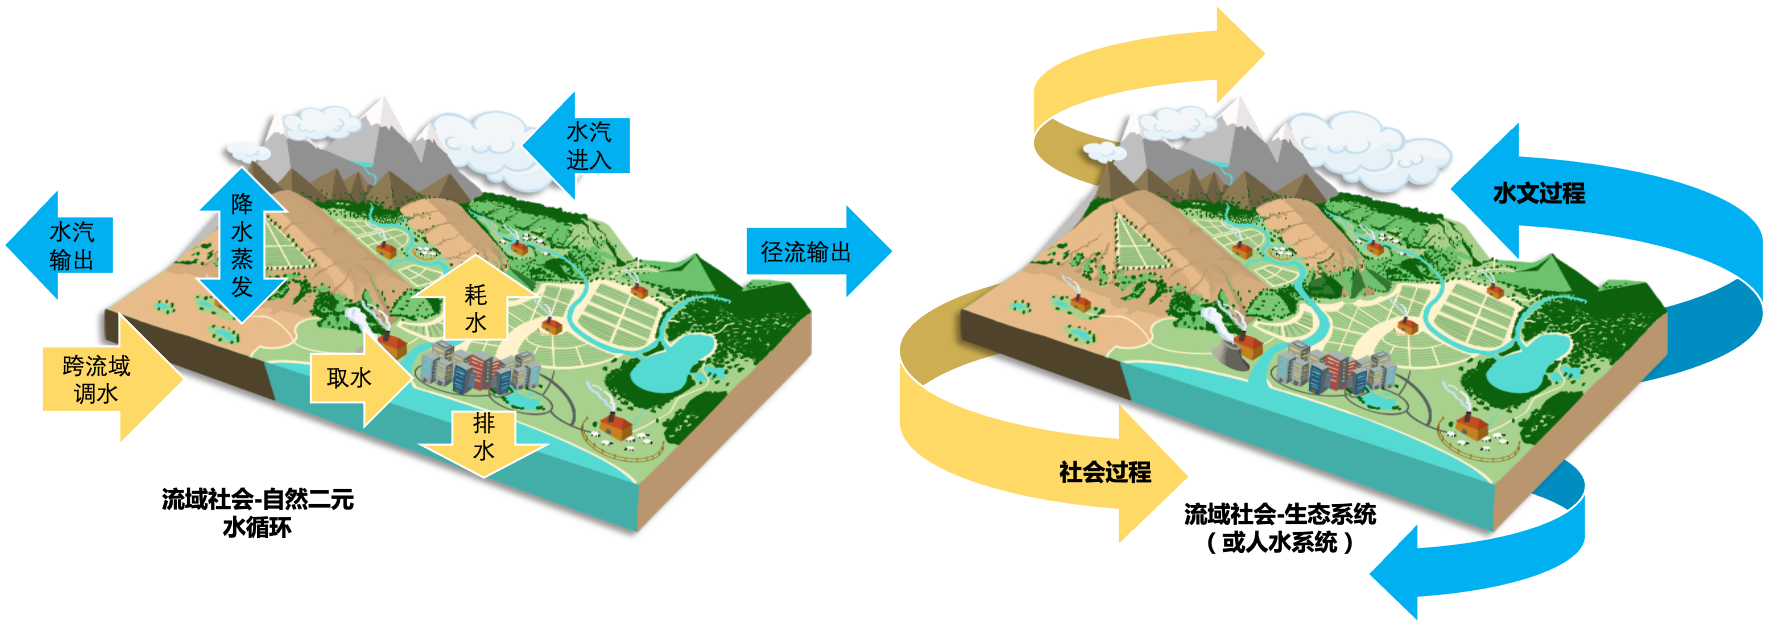
\includegraphics[width=\textwidth]{img/ch1/ch1_two_water_cycle.png}
    \caption[流域人水耦合系统的典型理论示意图]{流域人水系统耦合的典型理论示意图\cite{wang2006,dibaldassarre2015}。蓝色代表自然水循环的典型过程;黄色代表社会水循环的典型过程。}\label{ch1:fig:two_water_cycle}
\end{figure}

\subsubsection{社会-水文学}

% 开题报告
社会-水文学旨在理解人-水之间协同演化规律和循环互馈机制,多年来在现象检测、机理分析、模型预测等方面都获得了长足发展\cite{sivapalan2012, blair2016, srinivasan2016}。
社会-水文学在诞生之初便以流域系统为单元分析人与水的互动反馈过程(图~\ref{ch1:fig:two_water_cycle}右),其最根本的特征是将社会-水文系统视为动态系统,并将人类社会相关变量作为系统内部的驱动力,而非像传统水文学那样假设水文系统是在人类外部干扰下处于平衡态的\cite{sivapalan2012}。
Konar等人将社会-水文学的主要研究方向总结为四个:水循环与水资源利用、人与干旱之间的相互作用、人与洪水之间的相互作用、人与政策制度的相互作用\cite{konar2019}。
Yu等人则指出该学科经多年发展后呈现出三个特征:在水循环的不同时空尺度下开展研究、将人类文化的演化特征纳入研究、将基础设施建设对水循环的干扰纳入分析\cite{yu2020}。
在这种超越传统水文学的思想指导下,一些社会-水文现象得到揭示,例如增大用水效率却常常无法节约流域水资源的“用水效率悖论”\cite{grafton2018, xiong2021a},以及流域管理策略常在开发和保护之间周期性摆动的“钟摆效应”\cite{kandasamy2014, roobavannan2017, mostert2018}。

社会-水文学的发展同时也面临着诸多挑战。
Troy 等人通过文献分析,认为社会水文学研究尚集中在数据收集与整理、数据观察与推测、理论模型建立三个阶段,还缺乏对成熟的参数率定与模型预测,因此其预测能力相对较差,对指导政策制定还相去甚远\cite{troy2015}。
Sanderson 认为这种糟糕的模型表现很大程度上因为社会水文学并没有真正将社会因素纳入考量,因而发出了“社会-水文学需要社会科学”的呼吁\cite{sanderson2017}。
然而,社会科学常常没有统一、公认的理论,且人的主观能动性与文化变量均难以被模型捕捉。复杂系统的科学思想能够将复杂的人类行为纳入分析框架,被认为是社会-水文学未来重要的前进方向之一\cite{ahlstrom2021}。
综上所述,社会水文学的发展让人们对水问题背后的机制有了更深入的了解。分析与水相连接的社会动态是对传统的水文学的补充。但仍需要进一步在方法学上突破,结合多学科背景和复杂系统思想来分析社会-水文系统,以突破上述瓶颈。


\subsubsection{流域社会-生态系统}

% Handbook 什么是社会-生态系统
社会-生态系统的概念最早诞生于20世纪90年代中期,是生态经济学和公共池塘资源系统学者之间的跨领域研究,通过结合系统科学方法和适应性管理提出\cite{biggs2021},此概念有助于整合水的自然/社会属性研究\cite{fowler2022}。
它是一个典型的复杂适应性系统(complex adaptive system),由许多互相独立的部分组成,并以涌现的方式相互作用,系统层面的格局难以由某部分的属性来预测\cite{schluter2019}。
因此,社会-生态系统不等同于社会系统与生态系统的简单加和,而是由社会和生态组分之内/之间反馈所塑造的有机整体\cite{biggs2021}。
社会-生态系统理论发展至今已经产生了许多流行的框架,包括 Folke 和 Berkes提出的社会-生态系统概念框架\cite{berkes2008};将系统弹性描述为不同尺度适应性循环结果的扰沌框架\cite{gunderson2001};Liu 等人提出的远程耦合框架\cite{liu2018};Ostrom 分析公共池塘资源的社会-生态系统诊断框架\cite{ostrom2009};Schluter 等人提出的社会-生态系统行动情景框架等\cite{schluter2019}。

随着可持续发展目标的提出,社会-生态系统理论在21世纪得到广泛认可,作为跨学科概念反哺社会-水文学,逐渐形成了“流域社会生态系统”的概念。
Huggins对全球流域社会-生态系统在水资源压力下的脆弱性进行了评估,分析了淡水资源压力不断加剧对社会-生态系统的潜在影响,识别了全球的热点流域\cite{huggins2022}。
Varis综合考虑了社会系统的三种适应力和生态系统的三种脆弱性因素,在全球尺度评估流域社会-生态系统在弹性和适应之间的平衡\cite{varis2019}。
国内也逐渐接受流域系统是社会-生态系统或复杂系统的观点,重视系统科学在流域综合研究中的重要性。
程国栋和李新在“黑河流域生态-水文过程集成研究”中提出了流域科学的概念,将流域视为地球系统的缩微,考虑水文和生态系统的自组织性如何影响流域系统的功能,以及人的因素如何被集成到流域水文学和流域生态学中\cite{cheng2015}。
傅伯杰等人指出亟需聚焦人地系统耦合机理与调控途径,揭示黄河流域人水关系演变及社会-水文-生态系统动态\cite{fu2021a}。
一些实证研究也开始从不同角度分析流域社会-生态系统,包括结构变化\cite{song2022}、制度变化\cite{wang2019d}、社会意识\cite{liu2023}等对系统局部、流域系统、外部系统等产生的不同影响,证明了思想与社会-生态系统理论对流域研究的重要性。

\subsubsection{人水关系与人水系统}

正如中文语境的“人地关系”在英语世界一般等价于“human-environment interactions”\cite{li2016c, liu2023},“人水关系”直译的“human-water relationship”也并非英文世界的常见关键词,取而代之的是通常不限定时空尺度的术语“human-water systems”,即人水系统\cite{konar2019}。
人水系统是以水循环为纽带,将人文系统和自然系统联系起来并组成的复杂系统,能依靠自身循环动力和经济发展动力而演变\cite{zuo2007},也是一类典型的社会-生态系统,因此“流域社会-生态系统”与“流域人水系统”通常同义\cite{yu2020}。
左其亭认为中文语境常用的概念“人水和谐”不曾有严谨的学术定义\cite{zuo2007},指出“人水关系”应指人水系统中“人文系统”与“水系统”之间的关系,“人水和谐”则是对人水系统要素间关系的评价,并在此基础上提出了与“人水关系和谐论”与“人水关系学”\cite{zuoqiting2022, zuo2016a}。
但是,“人水关系学”侧重对人水系统进行整体评价,以指导水资源分配与流域管理,因此“人水关系”仍需被具体化为人类与水资源的多种互动关系\cite{zuo2016, zuo2020a}。

综上所述,许多理论框架,如“自然-社会二元水循环”、“社会-水文学”、“流域社会-生态系统”和“人水关系学”,从不同侧重点出发重视水的自然-社会双重属性研究。
其中,“自然-社会二元水循环”基于平衡态假设,已对多个流域在人类影响下的水平衡模式进行了计算与建模,服务于水资源管理工程;“社会-水文学”关注“人”与“水”之间的协同演化,在非平衡态假设下揭示了流域演变规律;“流域社会-生态系统”或“流域人-水系统”的概念结合了社会水文学与系统科学,强调整体性和协同演化的复杂性,是目前流域系统研究的前沿。
然而,目前流域尺度上仍缺乏对“人水关系”的具体定义,相关研究在不同时空尺度下均使用过于宽泛的“人水关系”概念,这给分析流域人水系统的演变过程与演变机制带来了阻碍。
鉴于在实际研究中,研究者绝无可能穷尽流域人-水系统的全部作用关系,本研究将“人水关系”的涵义界定为:人类活动直接改变水圈要素、过程,或人类决策反之受到水圈要素、过程不可被忽略的干预或影响时,人与地球表层系统的相互作用。


\subsection{人-水关系的演变过程}\label{ch1:sec:process}
协同演化路径的多样性体现了人水系统的复杂性,其演变过程也是流域社会-水文研究的热点。从侧重点不同可将目前研究分为“概念模式变化”、“关键指标变化”和“结构功能变化”三个方面。

概念模式是对许多共性规律的高度抽象或理论总结,以便研究人员和决策者在宏观层面把握人水系统的演变过程;关键指标则通过能够表征流域系统的关键变量或综合指标的变化规律来把握流域演变过程;而结构功能变化则是通过流域系统内重要组分的相互关系变化,以及与这种变化相关的系统功能改变来把握流域演变过程。

\subsubsection*{人水系统的概念模式变化}

在人水系统演变研究中,可以借鉴其他学科或领域的已有理论或概念,总结其概念模式的演变。
例如张家诚(2006)从科学哲史和科学哲学的角度出发回顾人水关系的演变历史,指出人水关系从古代时“天-地-人的平衡中庸模式”,到近代工业社会变为在追求自己的发展时忽略自然环境的“数学模式”,同时展望了信息时代人水关系的“工程调控模式”\cite{zhang2006}。
于宏瑞认为人-水关系是随着社会发展而变化的,因此经历了自然崇拜、趋势利用、盲目开发、持续协调四个阶段\cite{yuruihong2011}。
Gleick 和 Palaniappan 借鉴“石油峰值”为流域提出了“水峰值”的概念,借助该概念可将流域潜在水供应分为三个变化阶段:阶段一随着用水需求的增加可用水资源的供应(新修水坝、水库、泵);一旦达到最大成本效益的地表水和地下水开采;有一个最终转移到一个更高的成本支撑的供应水如海水淡化或转移等各种来源的增量增加供应\cite{gleick2010}。

人水系统演变的概念模式还可以通过流域的实际发展规律总结得出,这类模式通常有更活跃的理论生命力,也更能有助于指导后续研究和决策。
1999年,Turton提出了影响深远的“流域适应能力”概念框架,该框架指出,根据水资源的供需关系,流域人水系统随着发展可能依次在“获取更多水资源供应”、“提高用水效率”、“提高分配效率”、“适应水短缺状态”四种原型模式间演变\cite{turton1999}。
该框架在澳大利亚流域水治理改革案例中的应用不仅佐证了其重要指导意义,还暗示了流域演变过程可能还存在水需求下降的“第五阶段”\cite{loch2020}。
另一个典型的案例是通过澳大利亚东部 Murrumbidgee 河流域总结出的“钟摆效应”模式,它说明了流域人水关系在取水用于粮食生产和努力缓解流域环境退化之间保持动态演进,并在摇摆间将流域人水系统演变划分为四个时期\cite{kandasamy2014, roobavannan2017},而这一规律随后也在中国和欧洲等更多区域得到了复现\cite{han2017, mostert2018}。

\subsubsection*{人水系统的关键指标变化}

由于人水系统的复杂性,研究常从不同角度切入构建综合指标,用以表征人水关系的变迁。
刘海猛等人基于复杂自组织系统理论,在辨析人水系统基本内涵的基础上提出了人水关系演化的概念模型,将人水系统的演变过程概念化为社会经济、生态环境、水资源开发利用三个变量组的函数关系\cite{liu2014}。
Zuo 等人将“和谐人水关系”指标分为健康度、发展度、协调度\cite{zuo2008},该综合指标可将中国的人-水关系分为二十世纪中期以前、1950年至1980年、1980年至1990年、1990年之后四个时间阶段,各阶段的流域人水关系的主要特征分别是:应对用水需求和水灾、管理供水和去中心化、依法管理水资源、高度重视人水和谐\cite{zuo2016a}。

这种通过关键指标识别人水关系的方法须广泛收集来自不同领域的数据,在时间序列数据收集和数据同化上存在诸多挑战,但其优势在于一旦数据可用,能同时对全球各大流域进行大规模计算与分析。
Varis等人基于三个社会系统的适应性指标和三种生态系统的脆弱性指标,构建了综合指数评估流域社会-生态系统在弹性和适应之间的平衡,分析了各流域通过发展提升适应性的演变过程\cite{varis2019}。
Huggins等人则更侧重流域在水资源压力下的脆弱性,通过全球各流域的水资源可用性指标和人类面对压力的适应指标,综合分析了不断加剧的淡水资源压力对流域社会-生态系统的潜在影响路径\cite{huggins2022}。
Qin等人提出的稀缺性-韧性-易变性(SFV)指标,考虑了管理措施(如水库的建设)和用水结构变化(有些用水方式如能源用水是难以被短期替代的),选择了三个子指标对流域人类活动情况下水资源短缺情况做出评估,并分析了不同发展程度的地区在面对水资源短缺时的可能发展路径\cite{qin2019}。

\subsubsection*{人水系统的结构功能变化}

流域系统的结构变化是实现功能改变的必要条件,二者通常伴随着变化,因此寻找决定系统功能的关键变量,最直接的方式是通过结构变化识别流域人水关系演变。
例如,Wang等人提出了“矛盾统一”的人水关系理论框架,通过识别人与水之间是否是“对抗”关系,在两千年时间尺度上拟合了中国的人水关系变化\cite{wang2017}。
另一组常用于表征流域人水关系演变的要素是水、粮食和能源,但 Rollason 的研究指出,这三者之间的关系可能比许多研究中所表达的更为复杂\cite{rollason2021}。
因此,在利用关键要素间的关系进行识别时,需要精确把握关键变量,包括哪些要素需要纳入分析,以及如何构建它们之间的关系\cite{zhangzongyong2020, wang2021}。

改进上述问题的一个思路是使用复杂网络分析方法,尽可能考虑当前人水系统中所有需要考虑的因素,然后使用复杂网络指标分析系统演变\cite{sayles2019, bodin2017b}。
例如,Song 等人基于经济复杂性概念,使用全国的年均虚拟水足迹数据集(1978年至2008年)构建了农产品-虚拟水转移量的二分网络,通过复杂网络分析计算了网络复杂性随时间的变化,进而分析黄河流域水资源的重要性演变规律\cite{song2022}。
Sayles 等人结合生态和生态修复政策的数据,构建了流域的社会-生态网络,发现存在潜在结构问题的区域合作网络的密度和生产力都最弱的\cite{sayles2017}。
要识别网络结构,需要收集相对全面的关系数据集,并且对数据质量要求较高,这在一定程度上限制了此种研究方法的广泛应用。

最后,还可以直接从系统功能的角度出发寻找表征系统演变的证据,该方法易于在不同流域系统中使用,但依赖对人水系统功能的正确认识,因此得到广泛认可的方法指标相对较少。
Falkenmark 等人提出的“蓝水”和“绿水”概念\cite{falkenmark2006},以及后来提出的“灰水”,都是典型的从系统功能角度出发,研究流域结构-功能变化的理论框架\cite{mekonnen2011}。
传统水资源规划和管理针对的重点仅是河道的液态水(蓝水),大多数在流域面上以降水和蒸散的形式参与循环(绿水),此外还有少部分经人类利用后又参与循环的水资源(灰水),三者在流域人水系统中承担着截然不同的功能\cite{craswell2007}
随着流域社会经济发展和气候变化,流域水循环各部分的绿水和蓝水比例都会发生变化,这将对人水系统功能产生极为深远的影响,如降低弹性、削弱流域系统的生态系统服务、甚至导致系统崩溃\cite{falkenmark2019}。

综上所述,当前人水系统演变过程可以通过“概念模式变化”、“关键指标变化”、“结构功能变化”三个方面进行分析和总结,但仍需要加强三类框架之间的互相联系。如果流域人水系统的变化足够显著,上述三方面的研究理应是殊途同归的:通过识别关键指标变化的阈值,结构-功能表征系统整体变化,并对变化前后的系统状态做概念化总结。


\subsection{人-水关系的稳态转换}\label{ch1:sec:mechanism}
% 流域人水系统是典型的社会\textendash{}生态系统,系统演变机制是社会\textendash{}生态系统研究的核心内容。
% 根据侧重点的不同,武旭同将当前社会\textendash{}生态系统互馈的机制总结为“时”(系统弹性)、“空”(全程耦合)、“构”(结构匹配)、“阈”(地球界限)四个方面,其中“时”为包含弹性和稳态转换在内的一组概念,是研究社会\textendash{}生态系统动态演化的重要理论框架,对理解人水系统的演变机制至关重要\cite{WuXuTong2021}。
% 本节综述了与稳态转换密切相关的核心概念,并分别围绕“驱动因素、表现特征、级联效应”三个稳态转换的核心要素,总结了分析人水系统演变机制的主要路径。

\subsubsection{稳态转换与相关概念}

% 宋嘉熙 的 地理学报
弹性(Resilience)是指处于动态平稳的系统面对变化时通过缓冲、适应或转变等方式响应得以维持的能力\cite{folke2010}, 稳态转换(Regime shifts)指系统的结构和功能发生大规模重组并突破这种平稳状态的过程\cite{scheffer2001},在生态系统、气候系统、经济系统、及其它复杂系统中均可能发生,具有不易预测、难恢复的特点\cite{scheffer2003, biggs2009}。
通常使用“球-杯模型”或“折叠二分模型”来描述稳态转换。
以“球-杯模型”为例,不同稳态就像系统状态空间中凹陷的“杯子”,将系统实际状态则如同在不同凹陷间滚动的“小球”,状态空间的变化(参量驱动)或小球受到外力(变量驱动)时都可能推动系统状态在不同稳态间发生转换\cite{scheffer2009, folke2010}(图\ref{ch1:fig:regime_shift})。
稳态转换的诱发机制可以从参量驱动和变量驱动两个方面入手,前者是指外界条件(环境参数)发生变化时削弱系统弹性导致的稳态转换,后者是指系统内部或外部变量推动系统突破阈值从而触发的稳态转换\cite{scheffer2009, folke2010}(图\ref{ch1:fig:regime_shift})。
除了驱动因素外,系统稳态转换的发生可能致使系统功能与产出(Outcome)发生变化,或进一步触发其它的级联效应(Cascading Effect)\cite{rocha2018}。
因此,识别稳态转换应从“驱动力-现象-效应”这三个稳态转换的核心要素切入,从而厘清系统间反馈机理、分析关键要素间交互作用,揭示社会\textendash{}生态系统稳态转换的成因类型、现象特征与产出/外溢效应。

% Description of system regime shift by ball-cup model and fold bifurcation
\begin{figure}[!ht] % use float package if you want it here
    \centering
    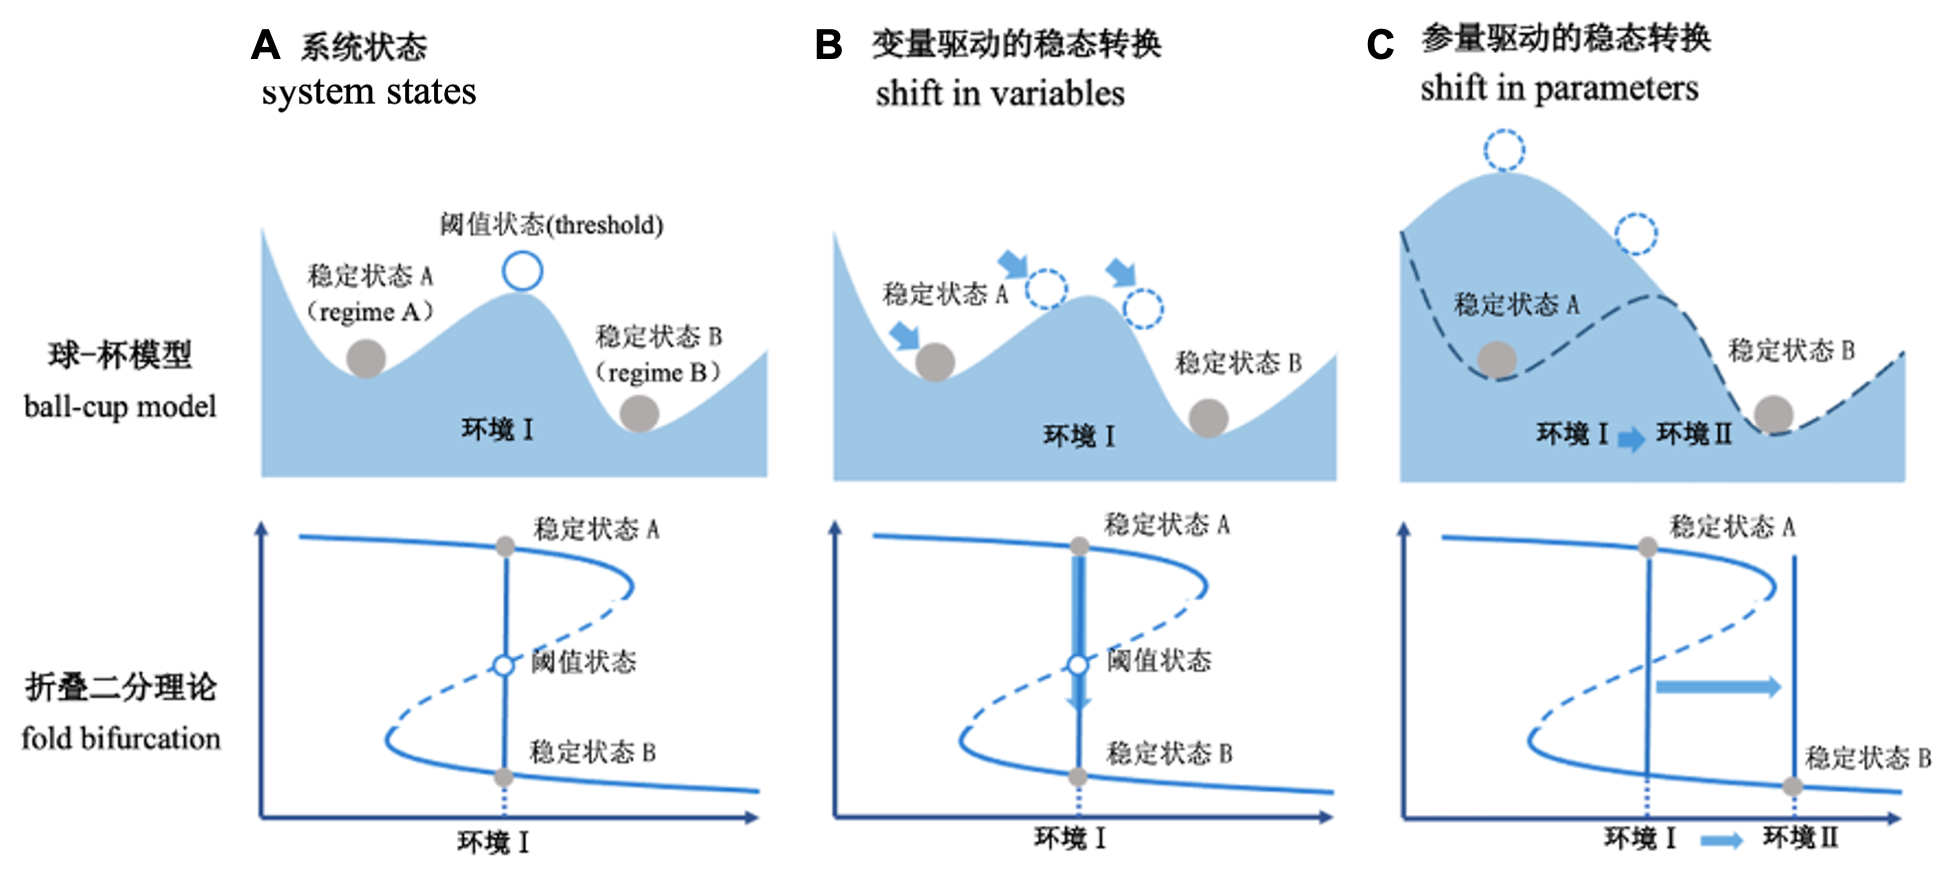
\includegraphics[width=\textwidth]{img/ch1/ch1_regime_shift.png}
    \caption[系统的稳态转换理论框架]{系统的稳态转换理论框架。
    \textbf{A}假设系统中存在稳定状态A和稳定状态B,球-杯模型(ball-cup model)和折叠二分理论(fold bifurcation)对系统各种状态的表征。
    \textbf{B}系统稳态转换过程。变量驱动的稳态转换(shift in variables):环境\romannumeral1不变时,处于稳定状态A的系统在干扰下自身突破阈值状态转换为稳定状态B。
    \textbf{C}参量驱动的稳态转换。环境\romannumeral1变为\romannumeral2,迫使处于稳定平衡状态A的系统向新环境下仅存的稳定平衡状态B转换。}\label{ch1:fig:regime_shift}
\end{figure}

\subsubsection{稳态转换的驱动因素}

Rocha等人发现,不断累积的人为干扰压力和气候变化是最常见的两类稳态转换驱动因素,无论以变量还是参量的形式出现\cite{rocha2018}。
Ji等根据水-沙调节方案和河口河道迁移这两个主要驱动因素变化的时间节点,结合不同阶段河口侵蚀-沉积量与河口排沙量,确定了河口侵蚀-积聚模式的稳态转换过程\cite{ji2018}。
Bao等在分析黄河中游水平衡系统稳态转换时,识别出气候驱动因素和土地利用/覆盖显著变化的阶段。通过验证不同阶段水平衡状态的差异确定了不同稳态阶段,并进一步定量解析了驱动水平衡状态转换的具体机制\cite{bao2019}。
此类分析路径的关键在于准确选择系统驱动力的定量表征,因此需要预设系统稳定状态和驱动力之间的关系。
这种方法多用于驱动力易于识别的干扰因素,如持续减少的林地、持续周期性变化的气候等。

“稳态循环”理论有助于理解另一类常见的人为干扰——流域治理措施——驱动的稳态转换。
该理论认为系统在不同尺度下都可以自组织历经适应性循环的“开发”、“保护”、“释放”、“更新”四个阶段\cite{gunderson2001},之后又进一步总结为“涌现”、“制度化”、“更新”三个阶段。
基于“主动改变不良的社会\textendash{}生态系统状态”与“调节并维持良好的社会\textendash{}生态系统状态”两种不同的目的,治理措施可分为自上而下的“转型治理”和自下而上的“协作治理”两类\cite{song2019}。
转型治理关注社会\textendash{}生态系统的释放和更新阶段,强调适应性治理的实现和主动促使社会\textendash{}生态系统完成状态的更新;协作治理则强调适应性治理制度化过程,旨在通过利益相关者间自组织的协作模式来实现社会\textendash{}生态系统的开发与保护\cite{song2019}。
因为无论自上而下或自下而上,流域治理既可能维持稳态,也可能触发稳态转换,需要在分析流域治理措施的作用机制时加以甄别。

\begin{figure}[!ht] % use float package if you want it here
    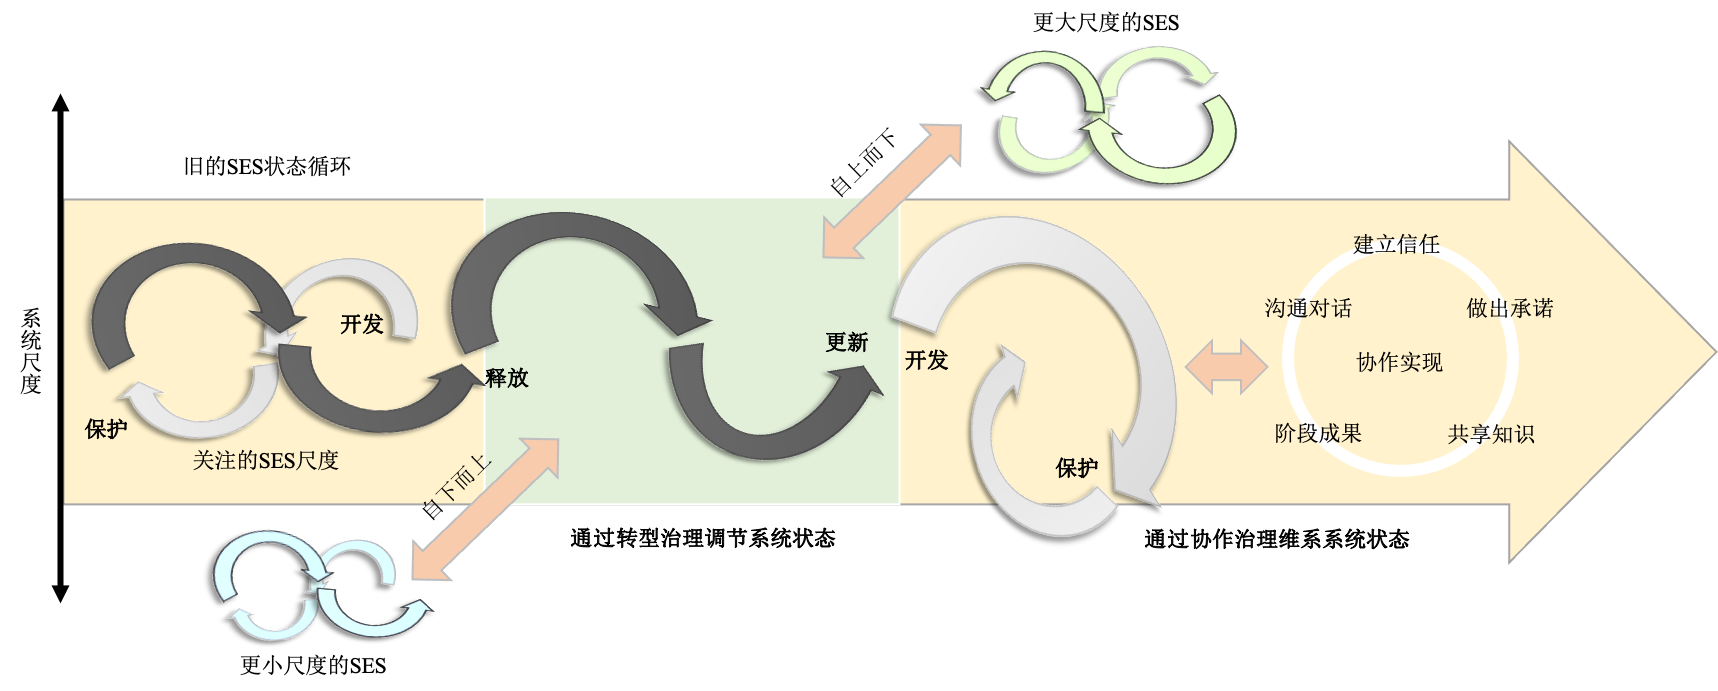
\includegraphics[width=\textwidth]{img/ch1/ch1_governance_driver.png}
    \caption[社会\textendash{}生态系统状态循环]{社会\textendash{}生态系统状态循环与转型治理、协作治理的关系。
    % Fig.4  The relationship between social-ecological system adaptive cycle and transition / collaborative governance
    图中展示旧的社会\textendash{}生态系统(SES)因转型治理而进入新的状态循环,并因协作治理的实现而延长开发保护阶段的过程}\label{ch1:fig:governance_driver}
\end{figure}

\subsubsection{稳态转换的表现特征}

聚焦于稳态转换过程中所表征出的现象是分析稳态转换最常见的路径,通过寻找合适的指标识别系统互馈变量或相关解释变量的趋势突变,检测稳态转换现象。
相关的检测方法非常丰富,常见的包括趋势分析、突变点检测或断点回归等。
Wang等利用t检验的循序算法和加性季节和趋势断点模型两种方法检测$1950 \textendash{} 2011$年黄河流域上中下游径流和输沙量的突变时间点以确定稳态转换时期\cite{wang2014};
Zhao等利用曼-肯德尔(Mann-Kenall)趋势分析法和加性季节和突变点检测模型识别出1921—2011年期间黄河月径流量趋势突变,重建天然径流量,量化人类活动对流量稳态转换的影响程度\cite{zhao2015}。

在识别稳态转换现象的基础上,还可以进一步将其与稳态转换驱动力相关联。
Yang等利用 Pettitt 检验计算稳态转换指数,探测流域径流的稳态转换,并与气候和土地利用变量的突变点对比分析,证实土地利用政策驱动了径流的稳态转换\cite{yang2012a}。
Niu等检测了黄河三角洲系统降水量,温度,月径流量和归一化植被指数(Normalized Difference Vegetation Index,NDVI)等多个现象相关变量共同的分解趋势断点,识别水文\textendash{}气候\textendash{}植被系统的稳态转换时期,分析各阶段内气候水文变量与NDVI间产出效应\cite{niu2020}。
虽然聚焦于稳态转换现象表征易于直观划分稳态转换的时期,且有着成熟的数据检测技术,但如果忽略对驱动和效应的结合分析,容易对稳态转换的驱动-响应机制表达不够全面。

\subsubsection{稳态转换的级联效应}

级联效应是指系统稳态转换后所产生的一系列后续影响,通过分析级联效应,可以更好地理解系统内部互馈关系的复杂性\cite{rocha2018}。
根据受到影响的要素在系统内或系统外,级联效应可分为内联效应和外溢效应\cite{rocha2018}。
在研究稳态转换时,Sun等利用沉积率曲线参数变化来刻画泥沙运输稳态转换的产出效应变化特征,同时解释了生态恢复对泥沙运输稳态的调节作用\cite{sun2020};
Wu等在研究黄土高原社会\textendash{}生态系统稳态转换时,通过量化社会\textendash{}生态系统内部要素交互作用的稳定状态,揭示了稳态转换不同阶段内系统关系变化和外溢效应\cite{wu2020a}。
Kidder等在研究黄河河道泥沙淤积系统稳态转换时,利用外溢系统中黄河下游洪水的频率和规模变化确定稳态转换发生时期,指出堤坝作为驱动因素对泥沙淤积存在着强烈正反馈\cite{kidder2015}。
此类分析路径有助于识别复杂的社会\textendash{}生态系统稳态转换的发生机制,正成为稳态转换实证研究的热点,但需要准确选择与系统反馈过程联系紧密的级联现象,因此也需要关于系统稳态的先验知识。

总的来说,虽然已有很多研究从驱动因素、表现特征和级联效应等不同方面探究人水系统的稳态转换机制,并提出了相应的量化方法,但稳态转换是大规模的系统重组,需要考虑多个要素的同步变化。
仅从单一要素出发的研究容易导致对其机制认识不全面,因此需要进行系统整合,探讨“驱动-现象-效应”的多要素联合变化。


\subsection{人-水关系建模}\label{ch1:sec:model}


% 开题报告
模型的建立是为了理解、描述和预测自然界,应当在真实性、预测性、普遍性之间达到均衡[27],流域系统模型通常旨在表征水的地球物理过程的动力学,以及人类用于管理系统的元素,如基础设施、机构和治理。 %\cite{hadjimichael2020}。
流域人水系统既有空间尺度依赖的地表生态过程,也有系统层次变量反馈的动力过程,还有多尺度的复杂人水相互作用[47–49]。
相应地,流域人水系统的建模主要有基于传统分布式水文模型耦合人类活动模块发展而来的分布式社会-水文模型、在系统或区域层次上耦合来自社会、自上而下模拟生态系统关键变量的系统动力学模型、自下而上对流域内复杂人-水互动进行仿真的多主体模型。

\subsubsection*{分布式社会-水文模型}

% 焦 本研一体 本子
与传统的集总式水文模型相比,分布式流域水文模型不再将流域视作均匀的整体,充分地考虑了流域内水文过程的异质性[207],是流域研究的主流工具,常见的分布式水文模型如如SWAT模型、新安江模型、陕北模型、布式时变增益水循环模型等(徐宗学,2019)[208-210],在国内外都得到了大量应用[211-213]。 % 焦 本子
% [207]王中根,刘昌明,吴险峰.基于DEM的分布式水文模型研究综述[J].自然资源学报,2003(02):168-173.
% [208]J. G. Arnold,R. Srinivasan,R. S. Muttiah,J. R. Williams. LARGE AREA HYDROLOGIC MODELING AND ASSESSMENT PART I: MODEL DEVELOPMENT[J]. JAWRA Journal of the American Water Resources Association,1998,34(1):73-89.
% [209]王中根,刘昌明,黄友波.SWAT模型的原理、结构及应用研究[J].地理科学进展,2003(01):79-86.
% [210]夏军,王纲胜,吕爱锋,谈戈.分布式时变增益流域水循环模拟[J].地理学报,2003(05):789-796.
% [211]Karim C. Abbaspour,Jing Yang,Ivan Maximov,Rosi Siber,Konrad Bogner,Johanna Mieleitner,Juerg Zobrist,Raghavan Srinivasan. Modelling hydrology and water quality in the pre-alpine/alpine Thur watershed using SWAT[J]. Journal of Hydrology,2006,333(2):413-430.
% [212]Darren L. Ficklin,Yuzhou Luo,Eike Luedeling,Minghua Zhang. Climate change sensitivity assessment of a highly agricultural watershed using SWAT[J]. Journal of Hydrology,2009,374(1):16-29.
% [213]Gangsheng Wang,Jun Xia,Ji Chen. Quantification of effects of climate variations and human activities on runoff by a monthly water balance model: A case study of the Chaobai River basin in northern China[J]. Water Resources Research,2009,45(7).
% 江 本子
流域分布式模型通过耦合生态过程,可用于描述大尺度流域陆地生态演变过程的生态水文模型,如SWIM模型(Krysanova等,2005)、RHESSys模型(Tague和Band,2004)、Budyko–Choudhury–Porporato模型(Donohue等,2012)、EHSM模型(Viola等,2014)、HYMOD-BGM模型(Tang等,2018)等。
国内的包括EcoHAT模型(刘昌明等,2009)、WEP-IBIS模型(Cao等,2015)、CLM-GBHM模型(Jiao等,2017)、GBEHM模型(Qin等,2017)、BEPS-TerrainLab模型(Chen等,2007)、HEIFLOW(Tian等,2018)等。

% 焦 本子
现有的分布式水文模型由于构建原理及最初率定区域不同,导致模型侧重点有所不同。如SWAT模型侧重描述产流过程[209],LISTFLOOD模型侧重模拟水动力过程、洪水过程等[217],但现有的分布式模型仍较少将人为干预水文过程的因素作为模拟重点,
% [209]王中根,刘昌明,黄友波.SWAT模型的原理、结构及应用研究[J].地理科学进展,2003(01):79-86.
% [217]曾照洋,王兆礼,吴旭树,赖成光,陈晓宏.基于SWMM和LISFLOOD模型的暴雨内涝模拟研究[J]
贾仰文等人WEP-L分布式流域二元水循环模型(简称 WEP-L 模型)是具有物理机制的流域分布式水循环模型,考虑了人类取用水和水利水保工程等因素对水循环过程的影响,实现“自然-社会二元水循环”过程耦合模拟和分析。 % todo citation
2019年,国际应用系统分析研究所(International Institute for Applied Systems Analysis, IIASA)开发了基于社区的水文模型模型(Community Water Model, CWatM)模型,将水库调度等水资源管理要素也纳入了模型[218]。
但迄今为止,仍鲜有将水资源治理制度(如法律法规)等人类活动要素的影响作为流域分布式模型模拟的重点。
% [218]Peter Burek, Yusuke Satoh, Taher Kahil,et al. Development of the Community Water Model (CWatM v1.04)- a high-resolution hydrological model for global and regional assessment of integrated water resources management[J].GEOSCIENTIFIC MODEL DEVELOPMENT,2020,13(7):3267-3298.

\subsubsection*{自上而下的系统动力学模型}

% 江本子
系统动力学模型能够自上而下地解析系统层面的要素关联、反馈与演化(Jaeger等,2017;Jiang等,2022),可预测变化环境下关键变量及其反馈过程的变化(Vaighan等,2017)。
许多大尺度的评估模型都是系统动力学模型,有 ANEMI3、 ANEMI Yangtze,以及在中国区域建立的 T21 China 模型,三者均包含自然和社会系统的多个部门,反映自然和社会系统的相互作用。
因此,流域人水系统的系统动力学模型可以通过分析系统间的相互作用、内部结构变化等现象,揭示流域人水关系的动态特征,如 ANEMI Yangtze 是在 ANEMI3 的基础上在长江流域建立的系统动力学模型。
将空间范围限制在流域尺度的系统动力学模型可以在建模过程中考虑研究区特征,使模拟结果更符合流域系统的实际情况,例如 ANEMI Yangtze 将长江的渔业作为模型的外生变量纳入考虑,分析了十年禁渔政策对流域系统的影响。 % todo citation

人类活动还可以作为系统内部反馈循环的关键变量被纳入模型。
% 开题报告
Viglione 和 Baldassarre 等人在流域尺度构建了用于解释和预测人类社会与洪水互相反馈、协同演化的系统动力学模型,其中水文要素(洪水)和社会组分(如公众意识、风险文化、经济发展等)都是反馈过程的核心变量[43]。
Muneepeerakul 等人(2017)则提出了一个流域社会-生态系统的发展轨迹模型,以探讨在什么情况下稳定的治理结构可以在促使堤坝等公共基础设施在系统中内生地出现\cite{muneepeerakul2017}。
系统动力学的劣势也很明显,首先是缺乏对空间特征的识别,这对流域系统是至关重要的;其次是通常需要自上而下对系统要素间关系给出基于数据或经验的函数假设,对于较为复杂且尚缺乏充分研究的流域系统变化,建模即便不是不可能,也将是非常困难的。

\subsubsection*{自下而上的多主体模型}
% 开题报告
涌现(Emergence)指系统实体会产生其所有组成部分本身没有的属性,人-水系统作为开放的复杂巨系统,广泛存在的相互作用就是宏观演化属性涌现的关键[51]。
% 来自 chat GPT
流域人水系统的多主体模型是指在研究人类活动对水资源的影响时,将不同的相关主体,如政府、水用户、环境保护者等作为系统的不同主体分别进行考虑,并综合考虑它们之间的相互影响关系,以达到更加全面、系统地研究人水关系的目的。这种模型在人水关系研究领域越来越受到关注,为了更好地研究人类活动对水环境的影响,并为流域水资源管理提供有力的指导。

自组织(Self-organization)是指一种起源于初始无序系统的部分元素之间的局部相互作用、所产生出某种形式的整体秩序的过程。这与复杂系统建模中自下而上的基于主体的建模(Agent-based model) 思想类似。
因此Castilla-Rho等人[61–63]利用多主体建模的复杂系统模拟方法将Ostrom发现的机制应用于地下水流域的管理模型中,发现可以解释地下水资源治理模式的涌现。但对于大河流域来说,由于人能直接观察到流动的水资源变化,且存在明显的时空分异性,尚缺乏较好的复杂系统建模以探索其中人-水关系的核心演化机制。

自下而上模拟流域水资源使用时上中下游不同行业利益相关者的冲突、合作,及其相互作用下治理体系的整理结构与功能,逐渐成为流域可持续治理的重要基础[53,54]。


刻画人水关系的模型和计量手段日益丰富,如应用多主体模型揭示了逐水而居的本能可能是人类早期迁徙演化的重要驱动力[42];

由于人类社会系统和流域水文系统的结构和功能具有不同的尺度和动态,匹配是指两者之间的良好关系。
Sayles 2017 研究了流域尺度社会-生态的匹配

总的来说,基于复杂系统的建模已成为研究人-水系统的重要技术手段,能够基于水的资源属性对利益相关者的人-水互动进行理论机制上的探索。这种自下而上的建模思路与SES的自组织管理机制一脉相承,但目前比较成熟的模型主要关注地下水流域和,对河流的水资源治理,尤其是水资源稀缺的大河尚缺乏泛用性较强的机制模型。


\subsection{黄河的人-水关系研究}\label{ch1:sec:yellow_river}

% 开题报告
黄河是全球人与水关系变化最频繁、最剧烈、影响最深远的大河之一。
人类社会与黄河相互作用的研究历史悠久,例如魏特夫对黄河流域的社会发展历史进行了考察,提出了著名的“水利社会理论”,认为这样的大规模的治水活动是中央封建王朝皇权诞生的重要因素\cite{weitefu1989}。
但许多中国学者认为,魏氏的观点是颠倒了复杂人-水关系中的因果关系,正是中央皇权的强劲发展使得大规模治水活动成为可能\cite{jizhaoding1981}。
治水策略的选择是决定黄河河道演变的重要人为因素,同时河道的自然条件也是选择治理策略的重要依据,由两者共同决定的治理结果会形成路径依赖\cite{WangWeiJing2009}。
因此,为了总结黄河流域人与水关系的变化,不乏有着眼于总结演变过程的著作。
于瑞宏详细地梳理了黄河流域人-水关系演变的典型事件,并将其分为上游、中游和下游区域,但未能将其串联在一起\cite{yuruihong2011}。
同样,有一些研究倾向于按照黄河流域人-水关系的关键主题来梳理演变进程,并努力展示其时间深度和因果关系,例如,葛剑雄从黄河与中华文明互动的角度进行了梳理\cite{gejianxiong2020},王渭泾则从黄河治理的角度进行了梳理\cite{WangWeiJing2009},以总结近两千年来黄河人-水关系的演变历史。
然而,这些研究通常仅限于对人水系统进行“专题梳理”,并以描述性概念模型为主,无法对流域人水系统的演变进行定量分析,因此难以满足对未来演变方向作出科学解释的需求。

% 于璐 本子
黄河流域是人-水关系和社会-水文学研究的重要案例。
长期以来,该流域受到人类活动的强烈影响,其人水关系演变具有复杂性,因此是稳态转换研究的代表区域\cite{zuo2022, wang2014}。
目前的研究主要集中在评估人类活动对流域的影响、评估人为干预治理或资源管理的效果与影响等方面\cite{wang2016a, WuXuTong2021, wang2019c}。
在分析人-水系统关系演变机制方面,一些研究集中在指标和结构层面,如耦合协调度\cite{libo2022}、承载力\cite{wang2022d}、多维指标评价\cite{li2020}、网络\cite{song2022}和蓝水与绿水等\cite{zhuo2016a}。
但这些方法依赖于对长期、结构化时间序列数据的收集,因此很难应用于分析非工程性质的、非连续的流域治理制度等人水系统驱动力的机制。
总的来说,黄河流域人-水关系演变机制的研究对于非工程的水资源治理措施的影响机制探讨不足,因此很难对流域规划中政策影响下的未来情景进行预测。

针对黄河流域人与水文系统的复杂关系,也有一些研究采用了同时考虑人类活动和水文过程的模型。
例如,贾仰文等人基于WEP模型开发了WEP-L模型,通过划分子流域和等高带的方法实现了黄河历史径流的复现\cite{jiayangwen2005}。
杨大文等人构建了分布式水文模型,以表示黄河流域的多个水文参数\cite{yangdawen2004}。
岳瑜素等人应用了系统动力学模型,优化了黄河下游滩区自然、经济和社会协同的可持续发展模式\cite{yueyusu2020}。
Jiang等人建立了系统动力学模型,从社会、经济、资源、生态和文化五个方面预测了在未来政策情景下黄河流域的高质量发展水平\cite{jiang2021b}。
黄昌硕等人建立了基于“经济社会-水资源-生态环境”系统动力学模型,为动态预测区域水资源承载力的变化趋势和制定优化调控方案提供了参考依据\cite{huangchangshuo2021}。
% 自己写的
相比于广泛发展和应用的分布式水文模型和系统动力学模型,仿真黄河复杂人水系统相互作用和揭示涌现现象的多主体模型研究相对较少。
Cai 在水资源调度方面使用了多主体模型,以优化黄河流域的水资源分配。然而,他模拟的主体数量较少,且主体间的互动仅考虑了工程要素,与水资源管理的联合多目标优化相似\cite{cai2011}。
Du 等人在黑河这个黄河的子流域实现了分布式水文模型和多主体模型的耦合,分析了水政策、农民用水和水文条件之间的关系,并指出了区域水文地质条件(如地下水位深度和与河流的距离)是影响人类与水文相互作用的关键因素\cite{du2020}。
但是,在黄河流域研究中,仍缺乏考虑多级利益相关者的、从下而上的、耦合分布式水文模型的多主体模型,限制了对不同政策情境下黄河人水关系演变机制的分析与预测。

总的来说,现有的研究主要集中于梳理黄河人水系统演变的概念模型,缺乏从流域人水系统视角出发的定量分析;尽管对演变机制进行了定量分析和建模仿真,但多集中在水库等工程因素的影响上,忽视了流域水治理政策对人水关系变化的重要驱动作用。


\section{研究目标与内容及关键科学问题}\label{sec:contents}

\subsection{研究目标}
% 武旭同话术,待修改
基于上述研究进展,本研究面向社会-水文学研究前沿,以黄河流域为研究区,结合水文气象观测、社会经济统计、历史数据重建、遥感反演等获取多源数据,借助统计分析和模型模拟等手段,分析黄河流域人-水关系的演变过程和驱动机制。具体研究目标如下:

(1)发展识别人-水关系演变规律的分析框架,分别在历史时期和现代治黄时期,揭示了黄河流域人-水关系演变过程、分析了不同阶段驱动流域人-水关系演变的主要原因。

(2)发展流域人-水关系演变机制分析的因果推断方法,建立黄河流域社会-生态系统的多主体模型,识别推动人-水关系变化的关键机制,定量评估其产生的影响。


\subsection{研究内容}

本研究具体包含以下主要内容:

% 开题报告
(1)黄河流域历史时期流域水沙特征演变:识别历史时期不断增强的人类活动压力超越气候周期变化的驱动力的时间,以及两者主导并推动黄河流域水沙特征突破临界点的稳态转换过程,分析该稳态转换发生之前黄河的人-水关系状态。
% 接下来利用建立的分析框架对黄河流域历史上的大事记进行分析,梳理出黄河流域人-水关系演变的主要脉络。最后利用系统回顾法,整合近代有研究以来对黄河人-水关系变化的定量分析成果,建立黄河流域人-水关系变化数据库,综合分析有研究以来人-水系统的主要驱动因素及演化路径。 

(2)现代治黄时期黄河流域的水治理演变:现代治黄的主要特征是强调流域系统综合治理,本研究分析上世纪六十年代以来黄河流域“稀缺情况、使用目的、分配方式”如何随时间变化,以及三者如何共同体现流域水治理变化,并解释这些变化背后流域系统如何被人类活动所主导。

(3)黄河流域分水制度变化的影响:在识别黄河流域现代水治理转变过程的基础上,分析治理转变期间,1987年和1998年两次流域水资源分配制度变化对流域系统的驱动机制,及其对社会-生态系统结构自上而下的重塑,定量识别该制度变化对流域不同地区用水的影响。

(4)黄河灌溉水分配的多主体建模:针对同样的制度变化过程,发展黄河流域粮食灌溉响应分水制度的多主体模型,模拟利益相关者对流域系统环境和制度变化的响应机制。自下而上分析粮食灌溉用水者对黄河流域水资源分配制度变化的适应过程,解析其用水来源对变化的响应。

其中识别历史时期的演变过程是理解人类活动如何主导流域人-水关系的关键,理解现代水治理转型是从工程治理走向综合治理的重要基础。后两部分主要内容则针对水治理转型期的典型非工程治理措施,从自上而下和自下而上的角度解析制度驱动人-水关系变化的效应与机制。基于上述研究内容,本研究的技术路线如图\ref{ch1:fig:workflow}所示:

\begin{figure}[!h] % use float package if you want it here
    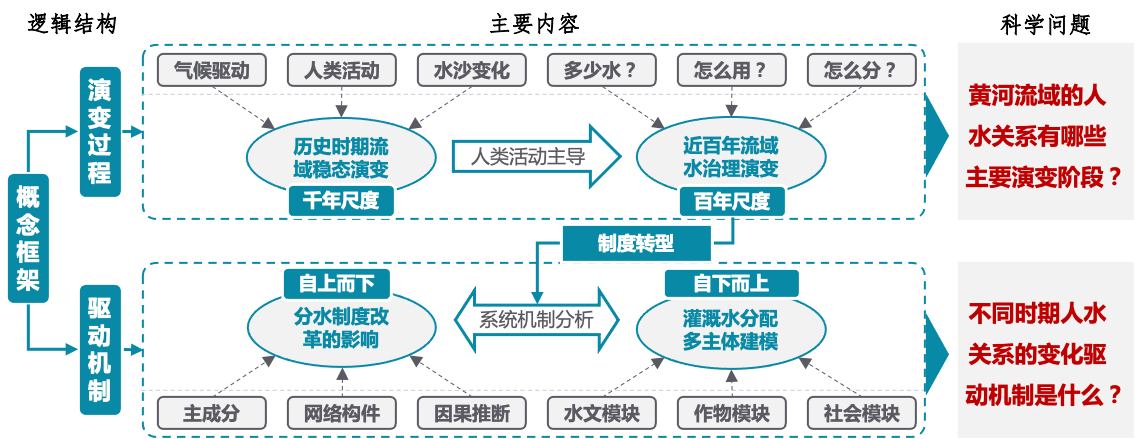
\includegraphics[width=\textwidth]{img/ch1/ch1_workflow.png}
    \caption{研究技术路线图}\label{ch1:fig:workflow}
\end{figure}

首先,针对历史时期和现代治黄的特点分别发展流域系统人-水关系演变的识别框架,厘定怎样的变化可以被识别为发生了“流域人-水关系演变”,以及有哪些潜在的驱动机制会导致这些变化,并总结黄河流域人-水关系的演变过程:
(1)人类主导流域水沙特征变化是黄河人-水关系变化的关键标志,黄河流域的水沙特征在历史时期发生从气候周期驱动向人类活动主导的过程。本研究使用历史重建资料和数据变化趋势识别病分析这一变化过程。
(2)水治理是现代流域人-水关系变化的主要驱动力,黄河流域的“自然-社会二元水循环”在现代治黄时期则已由人类活动主导,使用综合指标构建和突变点检测来识别流域水治理系统发生稳态转换的过程。
通过整合历史时期和人民治黄时期的人-水关系演变,可以回答“黄河流域的人-水关系有哪些主要演变阶段?”的科学问题,并总结各阶段黄河流域人-水关系的特征。

针对现代治黄时期流域治理转变由人类制度主导的特点,接下来的两章以制度变化为落脚点,以对黄河流域影响最为深远的水资源分配制度为例,分别从自上而下和自下而上两个路径分析流域人-水关系变化的驱动机制:
(1)自上而下:使用主成分分析、社会-生态系统网络构件识别、因果推断模型,分析制度变化对黄河流域系统结构及不同地区用水量的影响。
(2)自下而上:使用由人类模块和自然模块耦合构成的多主体模型,分析农业用水决策者的如何响应环境和制度变化,改变其水资源利用的过程。

\subsection{关键科学问题}

(1)黄河流域的人-水关系有哪些主要演变阶段?

(2)不同时期人-水关系变化的驱动机制是什么?


\section{研究区概况}\label{sec:study_area}
\subsection{黄河流域概况}

黄河流域($95^{\circ}52'37”$ \textendash{} $119^{\circ}3'56”E$,$32^{\circ}9'38”$ \textendash{} $41^{\circ}51'37”N$)跨越三个气候带,气候和生态系统类型复杂,干流流程$5.4 \times 10^3~km$、流域面积$76.6 \times 10^4~km^2$,约为中国国土面积的$8.3\%$,是中国第二长河。
黄河流域大部分位于我国干旱半干旱地区,年平均温度约为$6.4 ^{\circ}C$,潜在蒸发量超过$800~mm$,年均降水量不足$500~mm$且季节差异明显,中游以上流域夏季降水量可占全年降水量的$85\%$\cite{maxuening2012,wang2007}。
黄河流域地形变化较大,流域海拔变化超过$6200~m$,水面海拔高度差达$4480~m$。
流域内多样复杂的地形让黄河流域上、中、下游地理条件相差极大,且具有无以伦比的独特性:上游位于世界上最年轻/快速隆升的青藏高原;中游是唯一正在堆积/强烈剥蚀的黄土高原;下游供给着人口密集/水资源需求极大的华北平原。
上游与源区最重要的生态系统功能是水源涵养,黄河$534.79$亿立方米的多年平均地表水资源量中,有$60\%$以上来水来自兰州以上的源区\cite{huchunhong2018}。
中游黄土易垦区在人类活动和气候变化的双重影响下,因植被破坏和水土流失产生的泥沙让黄河曾以泥沙输运量最高的河流而闻名于世\cite{best2019}。
而在花园口站以下的黄河下游区域,因泥沙沉积抬高高程而形成了地上悬河,流域面积仅为$3 \times 10^4~km^2$,产流量低,且主河道在历史时期因频繁的洪泛决溢而在华北平原上频繁摆动,自西向东形成不计其数的辫状古河道。


\begin{figure}[!ht] % use float package if you want it here
    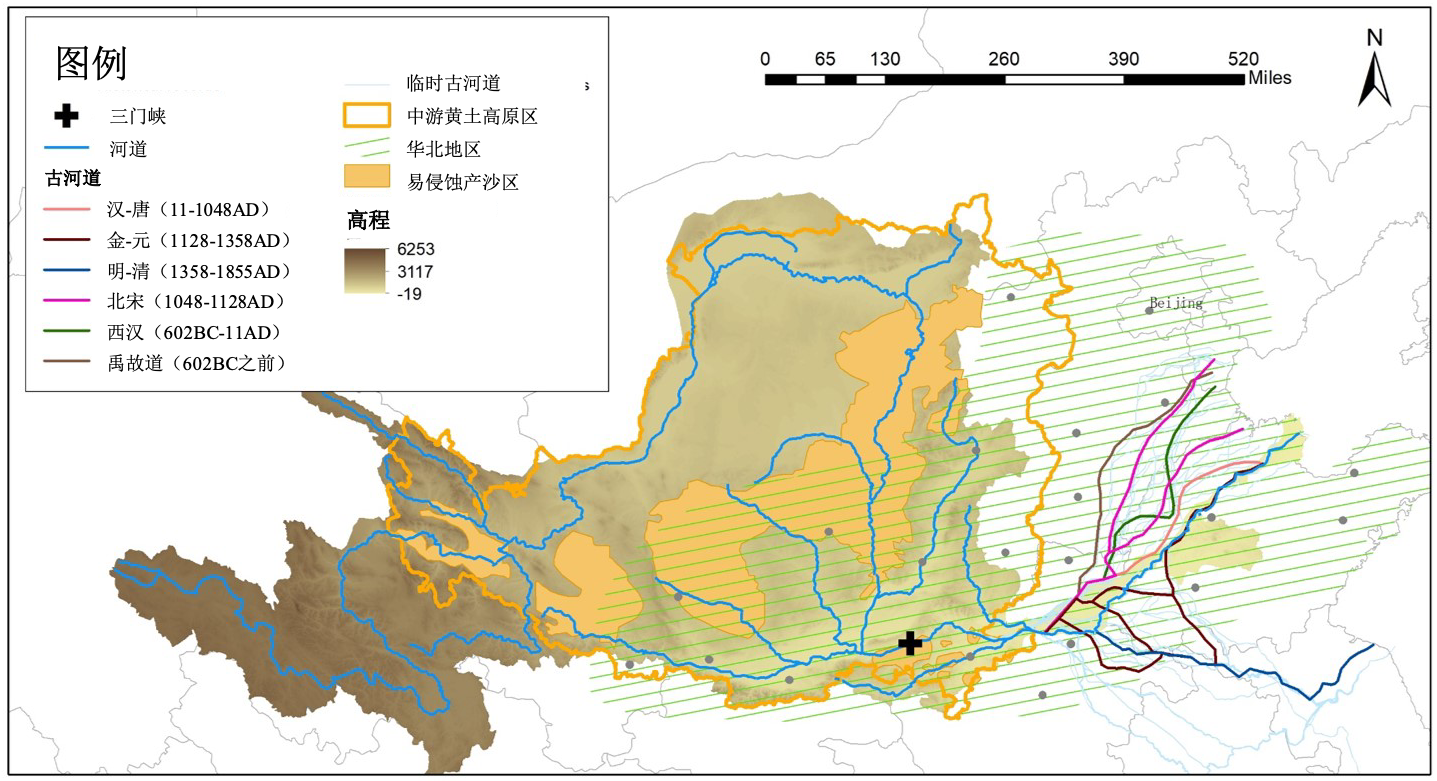
\includegraphics[width=\textwidth]{img/ch1/ch1_study_area.png}
    \caption{黄河流域研究区示意图}\label{ch1:fig:study_area}
\end{figure}

黄河流域历经了三千多年的开发和近现代的高强度经济活动影响,导致人类活动与资源环境之间的关系不断发生变化\cite{fu2021}。
随着人口的增长,中游黄土高原地区的耕种面积不断扩大,甚至发展到了丘陵和陡坡地区,造成了严重的水土流失,导致黄河的泥沙输送量急剧增加\cite{wu2020a}。
这些泥沙在下游堆积造成了地上悬河,导致洪泛决溢频繁发生,给黄河中下游的社会经济带来了灾难,例如宋朝和清朝都花费了大量的人力物力在黄河流域的救灾上。
从二十世纪中期以来,随着灌溉和水库技术的成熟,以及农业技术的进步,黄河下游逐渐从泛滥成灾变成了造福国家和人民的粮仓,但是同时也出现了“水少”的问题。
农业灌溉水资源的开发已接近极限,黄河的农业用水量占地表径流的超$70\%$,导致黄河自 $1972$ 年以来频繁断流,出现了日益严重的水资源危机~\cite{wang2019f}。
黄河流域是中国重要的农业和工业生产基地,人口稠密,社会经济活动密集。随着工业和服务业用水需求的增加,人-水-食物-能源的关系变得更加复杂,因此有必要根据人\textendash{}水系统的反馈循环,以长远和动态的眼光实现人\textendash{}水关系的和谐,以实现流域的高质量、可持续发展。

\subsection{黄河流域治理简史}

历史上,黄河流域的水治理一直是人\textendash{}水关系不断变化的重要驱动力。自有记录的历史以来,中央王朝就已经为治理黄河积累了大量的文献资料,并被视为关乎国家长治久安的重大任务。
在西汉中后期,随着河道淤积和河患增加,各种治河思想已经非常活跃。史料表明,在著名的“王景治河”时期,黄河下游已经普遍建有完备的堤防建设\cite{WangWeiJing2009}。
在王景治河之后,黄河流顺数世纪,直到北宋到元代重新进入了有史以来水患最严重的一段时期。频繁的河道变迁和堤防决溢迫使宋朝政府广泛征集治河水利人才,并建立岁修制度和治河责任制,但治河的总方针在“恢复东流”和“北流入海”之间的争执无法解决,因此国家大量的资金和粮食被用于河道作业和救灾\cite{WangWeiJing2009, yang2019}。
在明代,随着黄河泛滥的趋势逐渐缓解,河流治理主要是为了保护京杭大运河的漕运服务。当时采用了潘季驯的“束水攻沙”思想,初步认识到水沙关系的重要性\cite{WangWeiJing2009}。
在清朝前期,国力强盛时也有“汰沙澄源”的提议,重视水保,但未受到重视,因此政府仍然继续沿用古人思想进行治理,并将大运河与黄河分离,使漕运和治河并重。然而,随着清王朝中后期国力的逐渐衰弱,政府不再能承受这种黄河治理的压力,最终导致了又一次决堤,使黄河离开了七百年来南流夺淮的河道\cite{WangWeiJing2009}。


进入现代中国,科学认识的加深带来了“治黄先治沙”的治理方针,随后的一系列工程措施,如水库、淤地坝、渠道等,使得黄河的年平均泥沙输运量在六十年内降至原来的十分之一,缓解了困扰数千年的高输沙量和高淤积量问题\cite{wang2016a}。
面对水资源短缺等新的挑战,黄河流域采取了一系列有力的治理措施,包括工程措施(如水库联合调控、南水北调)和制度法规(如“水资源配额制度”、“最严格水资源管理”、《黄河流域保护法》等)\cite{shuilibuhuangheshuiliweiyuanhui2010}。
水资源配额制度对黄河流域的影响最为深远,从1980年首次提出到现在,它一直是指导和限制各地区用水的关键,比如联合调度、最严格水资源管理等都是在该方案的基础上执行的,但目前多个省份普遍认为该方案与实际情况越来越不符\cite{wang2019b,wang2019e}。
2019年9月的黄河流域生态保护和高质量发展座谈会上,黄河流域生态保护和高质量发展被正式定为国家重大战略,强调需要“重塑人\textendash{}水关系”和“坚守生态保护红线”。同年,黄河水资源分配制度的调整被列为当务之急;2022年,《黄河保护法》正式通过\cite{lu2019,dongzhanfeng2020}。
这些新举措表明,“治好黄河”的方向和决心一直没有改变。了解黄河流域人\textendash{}水关系的变化和机制,分析流域管理实践对人\textendash{}水关系的影响机制,将有助于在全球变化不断加剧的环境中,为黄河高质量和可持续发展提供科学依据。



\section{章节安排}\label{sec:chapters_summary}
